\documentclass[
	12pt,
	a4paper,
	bibtotoc,
	cleardoubleempty,
	idxtotoc,
	%ngerman,
	openright,
	final,
	listof=nochaptergap,
	]{scrbook}



% ##################################################
% Schriftarten und Zeichen
% ##################################################
\usepackage[T1]{fontenc}
\usepackage{lmodern}
\usepackage[utf8]{inputenc}
\usepackage[printonlyused,footnote]{acronym}
\usepackage{tabularx}
\usepackage{listings}
\usepackage{quoting}

% ##################################################
% Unterstuetzung fuer die deutsche Sprache
% ##################################################
%\usepackage{ngerman}
\usepackage[ngerman]{babel}

% ##################################################
% Dokumentvariablen
% ##################################################

% Persoenliche Daten
\newcommand{\docNachname}{Israel}
\newcommand{\docVorname}{Marco}
\newcommand{\docStrasse}{Am Wickenkamp 38}
\newcommand{\docOrt}{Stemwede}
\newcommand{\docPlz}{32351}
\newcommand{\docEmail}{Marco-Israel-Consulting@gmx.de}
\newcommand{\docMatrikelnummer}{242814}

% Dokumentdaten
\newcommand{\docTitle}{Embedded Linux}
\newcommand{\docUntertitle}{mit Yocto und OpenEmbedded}
%\newcommand{\docUntertitle}{} % Kein Untertitel
% Arten der Arbeit: Bachelorthesis, Masterthesis, Seminararbeit, Diplomarbeit
\newcommand{\docArtDerArbeit}{}
%Studiengaenge: Allgemeine Informatik Bachelor, Computer Networking Bachelor,
% Software-Produktmanagement Bachelor, Advanced Computer Scinece Master
\newcommand{\docStudiengang}{}
\newcommand{\docAbgabedatum}{Dezember 2019}
\newcommand{\docErsterReferent}{}
%\newcommand{\docZweiterReferent}{-} % Wenn es nur einen Betreuer gibt
%\newcommand{\docZweiterReferent}{ZWEITER REFERENT}

% ##################################################
% Allgemeine Pakete
% ##################################################

% Abbildungen einbinden
\usepackage{graphicx}

% Zusaetsliche Sonderzeichen
\usepackage{dingbat}

% Farben
\usepackage[usenames,dvipsnames,svgnames,table]{xcolor}

% Maskierung von URLs und Dateipfaden
\usepackage{url}

% Deutsche Anfuehrungszeichen
\usepackage[babel, german=quotes]{csquotes}

% Pakte zur Index-Erstellung (Schlagwortverzeichnis)
\usepackage{index}
\makeindex
%\usepackage[xindy]{imakeidx}

% Ipsum Lorem
% Paket wird nur für das Beispiel gebraucht und kann gelöscht werden
\usepackage{lipsum}


% ##################################################
% New commands
% ##################################################
\newcommand*{\fullref}[1]{\hyperref[{#1}]{\autoref*{#1} {Seite} \pageref*{#1}{;}
\nameref*{#1} }}
%\newcommand*{\namepageref}[1]{\hyperref[{#1}]{\nameref*{#1} \pageref*{#1} }}


% ##################################################
% Seitenformatierung
% ##################################################
\usepackage[
	portrait,
	bindingoffset=1.5cm,
	inner=2.5cm,
	outer=2.5cm,
	top=3cm,
	bottom=2cm,
	includeheadfoot
	]{geometry}

% ##################################################
% Kopf- und Fusszeile
% ##################################################

\usepackage{fancyhdr}

\pagestyle{fancy}
\fancyhf{}
\fancyhead[EL,OR]{\sffamily\thepage}
\fancyhead[ER,OL]{\sffamily\leftmark}

\fancypagestyle{headings}{}

\fancypagestyle{plain}{}

\fancypagestyle{empty}{
  \fancyhf{}
  \renewcommand{\headrulewidth}{0pt}
}

%Kein "Kapitel # NAME" in der Kopfzeile
\renewcommand{\chaptermark}[1]{
	\markboth{#1}{}
   	\markboth{\thechapter.\ #1}{}
}

% ##################################################
% Schriften
% ##################################################

% Stdandardschrift festlegen
\renewcommand{\familydefault}{\sfdefault}

% Standard Zeilenabstand: 1,5 zeilig
\usepackage{setspace}
\onehalfspacing

% Schriftgroessen festlegen
\addtokomafont{chapter}{\sffamily\large\bfseries}
\addtokomafont{section}{\sffamily\normalsize\bfseries}
\addtokomafont{subsection}{\sffamily\normalsize\mdseries}
\addtokomafont{caption}{\sffamily\normalsize\mdseries}

% ##################################################
% Inhaltsverzeichnis / Allgemeine Verzeichniseinstellungen
% ##################################################

% Control table of contents, figures, listings, etc
\usepackage{tocloft}

% Punkte auch bei Kapiteln
\renewcommand{\cftchapdotsep}{3}
\renewcommand{\cftdotsep}{3}

% Schriftart und -groesse im Inhaltsverzeichnis anpassen
\renewcommand{\cftchapfont}{\sffamily\normalsize}
\renewcommand{\cftsecfont}{\sffamily\normalsize}
\renewcommand{\cftsubsecfont}{\sffamily\normalsize}
\renewcommand{\cftchappagefont}{\sffamily\normalsize}
\renewcommand{\cftsecpagefont}{\sffamily\normalsize}
\renewcommand{\cftsubsecpagefont}{\sffamily\normalsize}

%Zeilenabstand in den Verzeichnissen einstellen
\setlength{\cftparskip}{.5\baselineskip}
\setlength{\cftbeforechapskip}{.1\baselineskip}

% ##################################################
% Abbildungsverzeichnis und Abbildungen
% ##################################################

\usepackage{caption}

\usepackage{wrapfig}

% Nummerierung von Abbildungen
\renewcommand{\thefigure}{\arabic{figure}}

% Abbildungsverzeichnis anpassen
\renewcommand{\cftfigpresnum}{Abbildung }
\renewcommand{\cftfigaftersnum}{:}

% Breite des Nummerierungsbereiches [Abbildung 1:]
\newlength{\figureLength}
\settowidth{\figureLength}{\bfseries\cftfigpresnum\cftfigaftersnum}
\setlength{\cftfignumwidth}{\figureLength}
\setlength{\cftfigindent}{0cm}

% Schriftart anpassen
\renewcommand\cftfigfont{\sffamily}
\renewcommand\cftfigpagefont{\sffamily}

% ##################################################
% Tabellenverzeichnis und Tabellen
% ##################################################

% Nummerierung von Tabellen
\renewcommand{\thetable}{\arabic{table}}

% Tabellenverzeichnis anpassen
\renewcommand{\cfttabpresnum}{Tabelle }
\renewcommand{\cfttabaftersnum}{:}

% Breite des Nummerierungsbereiches [Abbildung 1:]
\newlength{\tableLength}
\settowidth{\tableLength}{\bfseries\cfttabpresnum\cfttabaftersnum}
\setlength{\cfttabnumwidth}{\tableLength}
\setlength{\cfttabindent}{0cm}

%Schriftart anpassen
\renewcommand\cfttabfont{\sffamily}
\renewcommand\cfttabpagefont{\sffamily}

% Unterdrueckung von vertikalen Linien
\usepackage{booktabs}

% ##################################################
% Listings (Quellcode)
% ##################################################

%\usepackage{listings}
%\lstset{
%	language=java,
%	backgroundcolor=\color{white},
%	breaklines=true,
%	prebreak={\carriagereturn},
% 	breakautoindent=true,
% 	numbers=left,
% 	numberstyle=\tiny,
% 	stepnumber=2,
% 	numbersep=5pt,
% 	keywordstyle=\color{blue},
%   	commentstyle=\color{green},
%   	stringstyle=\color{gray}
%}

%\newcommand{\includecode}[2][c]{\lstinputlisting[caption=#2, escapechar=, style=custom#1]{#2}<!---->}
% Language define input
%\input{configs/listings-bash.prf}
%\input{configs/listings-C.prf}
%\input{configs/listings-C++.prf}
%\input{configs/listings-Python.prf}
%\input{configs/listings-Java.prf}


\lstset{
	language=bash,
	backgroundcolor=\color{gray},
    breaklines=true,                 % sets automatic line breaking
	prebreak={\carriagereturn},
 	breakautoindent=true,
    stepnumber=2,                    % the step between two line-numbers. If it's 1, each line will be numbered
    numbersep=10pt,                  % how far the line-numbers are from the code
    rulecolor=\color{black},         % if not set, the frame-color may be changed on line-breaks within not-black text (e.g. comments (green here))
    frame=single,	                 % adds a frame around the code
 	keywordstyle=\color{blue},
   	commentstyle=\color{green},
    stringstyle=\color{gray},        % string literal style
    numberstyle=\tiny\color{black},  % the style that is used for the line-numbers
    numbers=left,                    % where to put the line-numbers; possible values are (none, left, right)
    showspaces=false,                % show spaces everywhere adding particular underscores; it overrides 'showstringspaces'
    showstringspaces=false,          % underline spaces within strings only
    showtabs=false,                  % show tabs within strings adding particular underscores
    tabsize=2,	                     % sets default tabsize to 2 spaces
    title=\lstname                   % show the filename of files included with \lstinputlisting; also try caption instead of title
}


%\lstset{
%  backgroundcolor=\color{white},   % choose the background color; you must add \usepackage{color} or \usepackage{xcolor}; should come as last argument
%  basicstyle=\footnotesize,        % the size of the fonts that are used for the code
%  breakatwhitespace=false,         % sets if automatic breaks should only happen at whitespace
%  breaklines=true,                 % sets automatic line breaking
%  captionpos=b,                    % sets the caption-position to bottom
%  commentstyle=\color{green},      % comment style
%  deletekeywords={...},            % if you want to delete keywords from the given language
%  escapeinside={\%*}{*)},          % if you want to add LaTeX within your code
%  extendedchars=true,              % lets you use non-ASCII characters; for 8-bits encodings only, does not work with UTF-8
%  firstnumber=1000,                % start line enumeration with line 1000
%  keepspaces=true,                 % keeps spaces in text, useful for keeping indentation of code (possibly needs columns=flexible)
%  keywordstyle=\color{blue},       % keyword style
%  language=Octave,                 % the language of the code
%  morekeywords={*,...},            % if you want to add more keywords to the set
%  numbers=left,                    % where to put the line-numbers; possible values are (none, left, right)
%  numberstyle=\tiny\color{gray},   % the style that is used for the line-numbers
%  showspaces=false,                % show spaces everywhere adding particular underscores; it overrides 'showstringspaces'
%  showstringspaces=false,          % underline spaces within strings only
%  showtabs=false,                  % show tabs within strings adding particular underscores
%  stringstyle=\color{black},       % string literal style
%  tabsize=2,	                   % sets default tabsize to 2 spaces
%  title=\lstname                   % show the filename of files included with \lstinputlisting; also try caption instead of title
%}
%

% ##################################################
% Theoreme
% ##################################################

% Umgebung fuer Beispiele
\newtheorem{beispiel}{Beispiel}

% Umgebung fuer These
\newtheorem{these}{These}

% Umgebung fuer Definitionen
\newtheorem{definition}{Definition}

% ##################################################
% Literaturverzeichnis
% ##################################################

%\usepackage[
%]{bibgerm}

\usepackage[backend=biber, %% Hilfsprogramm "biber" (statt "biblatex" oder "bibtex")
%style=authoryear, %% Zitierstil (siehe Dokumentation)
style=alphabetic,
%style=numeric,
%style=ieee,
natbib=true, %% Bereitstellen von natbib-kompatiblen Zitierkommandos
hyperref=true, %% hyperref-Paket verwenden, um Links zu erstellen
]{biblatex}

\addbibresource{bibtex} %% Einbinden der bib-Datei

% ##################################################
% PDF / Dokumenteninternelinks
% ##################################################

\usepackage[
	colorlinks=false,
   	linkcolor=red,
   	citecolor=green,
  	filecolor=magenta,
	urlcolor=cyan,
    bookmarks=true,
    bookmarksopen=true,
    bookmarksopenlevel=3,
    bookmarksnumbered,
    plainpages=false,
    pdfpagelabels=true,
    hyperfootnotes,
    pdftitle ={\docTitle},
    pdfauthor={\docVorname~\docNachname},
    pdfcreator={\docVorname~\docNachname}]{hyperref}



% ##################################################
% Glossrry
% ##################################################
    %\usepackage[nomain,acronym,xindy,toc]{glossaries}
    \usepackage[acronym]{glossaries}
    \setglossarystyle{listhypergroup}
    \makeglossaries
    \loadglsentries{content/glossary} %Glossary in externer Datei...



\begin{document}

% ##################################################
% Definitionen neuer Befehle
% ##################################################

\newcommand{\bb}{$\backslash$} %Backshlash


\setcounter{secnumdepth}{3}

% ##################################################
% Titelblatt
% ##################################################
%\begin{titlepage}
\pagestyle{empty}

% ##################################################
% HFU-Logo einbinden
% ##################################################
\begin{flushright}
\begin{figure}[ht]
\flushright

\includegraphics[height=3cm]{pictures/logo.png}
\end{figure}
\end{flushright}

% ##################################################
% Titel
% ##################################################
\begin{center}
%{\fontsize{18}{22} \selectfont \docArtDerArbeit}\\[5mm]
%{\fontsize{18}{22} \selectfont im Studiengang} \\[5mm]
%{\fontsize{18}{22} \selectfont \docStudiengang}\\
\vspace{1cm}
\begin{onehalfspace}
{\fontsize{22}{26} \selectfont \textbf{\docTitle}}\\[5mm]
{\fontsize{18}{22} \selectfont \docUntertitle}


\end{onehalfspace}
\end{center}

% ##################################################
% Zusatzinformationen
% ##################################################
%\vfill
%\begin{center}
%\begin{tabular}{lcl}
%Referent  		&:& \docErsterReferent 	\\ \\
%Koreferent 		&:& \docZweiterReferent \\ \\
    \begin{center}
        Von \docVorname~\docNachname\\
 	    \docAbgabedatum
    \end{center}
%				& & Matrikelnummer: \docMatrikelnummer\\
%				& & \docStrasse,~\docPlz~\docOrt	\\
%				& & \docEmail
%\end{tabular}
%\end{center}
\end{titlepage}


\cleardoubleemptypage{}

\frontmatter


% ##################################################
% Abstract
% ##################################################
%\include{content/abstract}
\cleardoubleemptypage{}


% ##################################################
% Inhaltsverzeichnis
% ##################################################
\tableofcontents
addcontentsline{toc}{chapter}{Inhaltsverzeichnis}
\cleardoubleemptypage{}


% ##################################################
% Abbildungsverzeichnis einbinden und ins Inhaltsverzeichnis
% ##################################################
% WORKAROUND: tocloft und KOMA funktionieren zusammen nicht
% korrekt\phantomsection
\addcontentsline{toc}{chapter}{\listfigurename}
\listoffigures
\cleardoubleemptypage{}


% ##################################################
% Tabellenverzeichnis einbinden und ins Inhaltsverzeichnis
% WORKAROUND: tocloft und KOMA funktionieren zusammen nicht
% korrekt\phantomsection
% ##################################################
\phantomsection{}
\addcontentsline{toc}{chapter}{\listtablename}
\listoftables
%\cleardoubleemptyp
%\usepackage[printonlyused]{acronym}


% ##################################################
% Abkürzungsverzeichnis
% ##################################################
\chapter{Abkürzungsverzeichnis}
\begin{acronym}
    \acro{SDK}{Software Development Kit}
    \acro{DTB}{Device Tree Blob}
    \acro{BSP}{Board Support Packed}
    \acro{TFTP}{Trivial File Transfer Protocol}
    \acro{NFS}{Network File System}
    \acro{FTP}{File Transport Protocol}
    \acro{WYSIWYG}{What you see is what you get}

    \acro{PDF}{Portable Dokument Format}
    \acro{HFU}{Hochschule Furtwangen}
    \acro{ISO}{International Organization for Standardization}
    \acro{AES}{Advanced Encryption Standard}
    \acro{RC4}{Arcfour}
    \acro{ASCII}{American Standard Code for Information Interchange}
    \acro{XRef}{Cross Referenz}
    \acro{HTTP}{Hypertext Transfer Protocol}
    \acro{OLE}{Object Linking and Embedding}
    \acro{EOL}{End of Line}
    \acro{EOF}{End of File}
    \acro{MD5}{Message-Digest Algorithm Version 5}
    \acro{SHA}{Secure Hash Algorithm}
    \acro{ES}{Escaptes Sonderzeichen}
    \acro{SZ}{Sonderzeichen}
    \acro{FDF}{Forms Data Format}
    \acro{PJDF}{Portable Job Ticket Format}
    \acro{HTTP}{Hypertext Transfer Protocol}
    \acro{CMYK}{Cyan, Magenta, Yellow und der Schwarzanteil Kay}
    \acro{RGB}{Rot, Grün und Blau}
    \acro{VDP}{Variable Data Printing}
    \acro{PAdES}{PDF Advanced Electronic Signatures}
    \acro{SP}{Space Character}
    \acro{HT}{Horizontal Tabulator}
    \acro{CR}{Carriage return}
    \acro{LF}{Line feed}
    \acro{FF}{Form feed}
    \acro{NUL}{Null character}
    \acro{OID}{Object Identifier}
    \acro{ETSI}{European Telecommunications Standards Institute}
    \acro{VM}{virtuelle Maschine}
\end{acronym}


%\printglossary[type=\acronymtype,title=Acronyms and
%Abbreviations,toctitle=Abbreviations]



% ##################################################
% Content
% ##################################################

\mainmatter{}
\chapter{Introduction}\label{chp:einleitung}
The control panel (CP) for the Telair International GmbH cargo loading system is
a client-server system communicating over an CAN interface. The control panel is
the client which gets input from buttons and switches, displays the action on an
LCD and sends information over to the server. On the client system an Linux
system is running, iterating between User input and handles the tasks  to be
preformed.  Only the client system from the Software side is descried in this
document.

\section{About the Linux Kernel}%\label{sec:About the Linux Kernel}

A mainline \textbf{Linux kernel version 4.4.39} is running on this hardware.
This kernel version is compatible to the last release of \textbf{\gls{BSP}
packet version 119} supporting the last \textbf{tqma335x module revision 2.2.3.}
The used \gls{BSP} was released in Dezember 2019. To be compatible to this
BSP was the reason choosing this kernel version and not a current Linux kernel
like 5.x.

Some changes were made to the Linux mainline Kernel like replacing the \gls{DRM}
video drivers to get the LCD running according to the TI
errata~\cite{TI_am335x_errata} as well as changes in the Kernel configuration.

The howl changes made to mainline kernel provided by the TQ BSP packet version
119~\cite{tq_bsp119} are described during the following chapters inside this
document. \textbf{That is what this document is about}.
\chapter{Basics}% \label{cha:Basics_and_general_information}
\section{About PTXdist}%
\label{sec:linux_distribution_build}

How to \textbf{install PTXdist}, how to \textbf{use it} and how to to build the
final Linux distribution configured by use use of PTXdist is in detail descried
online on websites. \textbf{This section provides the information where to find
    online descriptions compatible to the tqma335x chip}.


\subsection{PTXdist setup}% \label{sub:PTXdist setup}
To setup PTXdist you need to preform the following steps online documented.

\begin{description}
    \item[To build the Linux distribution] the framework \textit{PTXdist} is
        used. Refer to \newline \textbf{\cite{ptxdist}} to get an introduction
        to PTXdist.
    \item[How to install PTXdist] and get this framework running, is descried in
        \textbf{\cite{tq_bsp119_install}}. You find here how to setup your
        build host (requirements to the building host) and how to install the
        \textbf{right} (compatible) \textbf{cross compiler version}.

        \textbf{ATTENTION:} You should read the \textbf{WARNINGS} from TQ
        carefully to get the right ordering of installation and setup.

        \textbf{ADDITIONALLY} you should take a look into the
        \textbf{\cite[PTXdist installation guide]{ptxdist_install} }
        to get information not described by TQ and to realize what is spacial
        to TQ.\@
    \item[How to setup TQ Systms BSP] for the base chip (like tqma335x)
        is described in short by TQ systems. Refer to
        \textbf{\cite{tq_bsp119_configuration}} and follow the instructions to
        setup the project environment. You need to prefome the steps there for
        BSP Revision up to v117. Here an example of steps to preform true for
        the BSP Version used in this Project.
\end{description}

\subsubsection{Setup for this pre-installed machine }%\label{ssub:this_setup}
In order to setup a new project by using this pre-installed machine with the
same BSP version, here an example of steps to setup the new project as it was
done for this project.

\begin{itemize}
    \item You can call a simple setup script by TQ:\@
        Run from From your <projetroot> (see \fullref{cha:locations})
        \begin{lstlisting}[language=bash, gobble=12,caption={Run TQ-Systems
        enviroment setup script}]
                user@machine: ./tools/config-tqma335x.qt4
        \end{lstlisting}

    \item You also can also manual select a needed configurations as follows:

        \begin{description}
            \item[Select a Software configuration] run from inside <projectroot>

                \begin{lstlisting}[language=bash,gobble=12, caption={Select the
                ptxdist configuraion file},keywordstyle=\color{black}]
            user@machine: ptxdist select ./configs/platforms/tqma335x/mba335x/platformconfig
                \end{lstlisting}~\cite[Selecting a Userland
                Configuration]{ptxdist_manual}

            \item[Select a Hardware configuration] run from inside <projectroot>

                \begin{lstlisting}[language=bash,gobble=12, caption={Select the
                ptxdist configuration file.}]
            user@machine: ptxdist platform ./configs/systems/qt/ptxconfig
                \end{lstlisting}
                You can take a look at~\cite[Selecting
                a Hardware Platform]{ptxdist_manual}
            \item[Select a toolchain]
                The toolchain should be autoselected. If not take do it
                manual
                \begin{lstlisting}[language=bash,gobble=12,caption={Select the
                cross compiler toolchain}]
            user@machine: ptxdist toolchain '/opt/<path-to-your-toolchain/bin'
                \end{lstlisting}
                You can take a look at~\cite[Selecting a Toolchain]
                {ptxdist_manual}
        \end{description}


    \item Finally after preforming one of above steps run a clean default build
        from inside your <projectroot>:
        \begin{lstlisting}[language=bash,gobble=12,caption={Initial PTXdist
        build}]
            user@machine: ptxdist go --git
                #[..downloading and build default packes, kernel bootloader...]
            user@machine: ptxdist images
                #[...building all activated image types ...]
        \end{lstlisting}
\end{itemize}



\subsection{PTXdist usage}%\label{sub:ptxdist_usage}

The online manual~\cite[PTXdist user manual]{ptxdist_manual} descries the basic
usage of PTXdist. Here the chapter \textbf{\#first-steps-with-ptxdist} is for
you of interest. You can also take a look into~\cite{ptxdist_developer} if you
have more special questions, e.g. \textit{like how to reconfigure and recompile
the Linux kernel via PTXdist} or into the~\cite[PTXdist FAQ list]{ptxdist_faq}
(which of course is very short). The most important commands you will need are:

\begin{description}
    \item[Prefome all steps] and finally build the images all in one
        command
        \begin{lstlisting}[language=bash,numbers=none,caption=Build all
        images with PTXdist]
        user@machine: ptxdist images
        \end{lstlisting}
    \item[Deleate a paket]. This is important before you like to rebuild it.
        Especially if you modify on of the configuration files (see next
        command).

        \begin{lstlisting}[language=bash,numbers=none,caption=Deleat a
        builded packet from PTXdsits scope]
        user@machine: ptxdist clean <your-packet>
        \end{lstlisting}
\newpage
    \item[Alter one of the configuration files] (see~\cite[PTXdist user
        manual]{ptxdist_manual}).

        The most important ones are:

        \lstset{style=bash}
        \begin{lstlisting}[language=bash,numbers=none,caption=Alter a
        configuration]
            #PTXdist main configuration
        user@machine: ptxdist menu
            #Project configuration
        user@machine: ptxdist menuconfig
            #Platform configuration
        user@machine: ptxdist platformconfig
            #Linux kernel configuration
        user@machine: ptxdist kernelconfig
        \end{lstlisting}
    \item[(Re-) Compile] a packet see~\cite[PTXdist’s build
        process]{ptxdist_manual}.

        Here an example if you like to extract, compile, configure, patch and
        install a new packed into the targets \gls{rootfs} all in on step you can
        run:

        \begin{lstlisting}[language=bash,numbers=none,caption=Compile and
        install a paket with PTXdist]
        user@machine: ptxdist targetinstall telair-cp_790760_1
        \end{lstlisting}

        Where \textit{ptxdist-cp\_790760\_1} is the \textit{ptxdist rule name}
        describing how to handle packet packets to build. For more details refer
        to~\cite[PTXdist development guide]{ptxdist_developer}.
\end{description}

\subsection{Extends and modify the basic project }%
\label{sub:extends_project}

If you need to extends the current project e.g.\@ by new software packages or an
new project, you should read the following guides:
\begin{description}
    \item[How to extend PTXdist] is descried motley in the
        \textbf{\cite[developer guide]{ptxdist_developer}}. Some extend
        information and \glspl{FAQ} are descried in
        \textbf{\cite{ptxdist_workflows}}, by other websites in the internet
        or if you write your supplier or like TQ Pengutronix an e-mail.

    \item[Background how PTXdist works] is described in the~\cite[PTXdist Users
        Manual]{ptxdist_manual} in the chapter \textbf{\#how-does-it-work}.
\end{description}


\section{Git}%
\label{sec:git}
Git is a distributed (and also central) version control system which only saves
changes to a file instead of copies. Switching between development versions is
easy this way. Additional Git has a lot of other features compared to other
\glspl{VCS} systems. Git was developed 2005 by Linus Torvalds.

Followings are links to tutorials and description which descries what git is,
what its benefits are  and how you can use it.


\begin{description}
    \item[The Git referance] is available in~\cite{gitdoc}. This gives
        an overview to the possible Git command and its meaning.
    \item[An Open PDF book] provided by the git homepage:~\cite{Chacon2014}. It
        also holds an command index on the last side like the online
        documentation mentioned out above. Thanks to PDF and linkage you
        can directly jump to the descriptions with examples and well designed
        pictures. Below is a video series which shows some of the examples and
        pictures inside this book.
    \item[A Video tutorial series] by an English
        speaker:~\cite{gitvideotutorial_en}.
        He orients on the book mentioned out above and gives examples and
        pictures you find inside this books.
    \item[A Video tutorial] (English) by an German
        speaker:~\cite{gitvideotutorial_de_en}
    \item[A Cheat-Sheet] gives an overview with a short descriptions of the most
        used git commands and git commands flags:~\cite{git_cheat_sheet}. You
        can download it as PDF.\@ The website also give some practical examples
        with command line pictures to some of the commands and workflows.
    \item[The Picture of Git states] gives an overview of the local and remote
        repositories philosophic behind git and shows corresponding
        commands~\cite{git_picture}
\end{description}

\chapter{Locations}%
\label{cha:locations}

\section{Project relevant files inside the PTXdist build machine}%
\label{sec:relevant_files}


Here is brave overview over the locations where to find recent files belongs to
this project and the Telair International GmbH inside the Virtual Box Linux
machine and inside the PTXdist project.

\begin{description}

    \item[The PTXdist project itself] is located inside the \gls{VM} at:

        \begin{alltt}
        \textit{/ptxdist/projects/cp790760}
        \end{alltt}

        \textbf{This location is the \textit{project-root}} as it will be called
        further on inside this documentation.

    \item[Source files downloaded by PTXdist] like the Linux kernel or software
        packets can be found in:

        \begin{alltt}
        \textit{/ptxdist/sources}
        \end{alltt}

        This folder could be
        used as a global source folder for other projects if you are using this
        VM again. Its also possible to locate \textit{Yocto} to it.

    \item[The cp790760 software sources] are located in:

        \begin{alltt}~\label{part:location_cp790760_software}
        \textit{<project-root>/local\_sources/telair-cp\_790760\_1 }
        \end{alltt}

        PTXdist is compiling this sources during the build project and will
        place it into the SDCard rootfs.

    \item[The cp790760 data files] like pictures or configuration files, are
        located in:
        \begin{alltt}
        \textit{<project-root>/local\_sources/
        \qquad\(\hookrightarrow\) telair-partion-files/partion-data/files}
        \end{alltt}
        This are the files which will be placed in the so called \textit{data}
        partion on the SDCard.

    \item[The cp790760 log files] are located in:
        \begin{alltt}
        \textit{<project-root>/local\_sources/
        \qquad\(\hookrightarrow\) telair-partion-files/partion-log/files}
        \end{alltt}
        This files are old log files. This mechanism to copy old log files is
        only if you like to update the system and want to hold the old logs.
        Otherwise the running system will create new files after the systems
        boots the first time.

    \item[The Telair specific hardware description] which is needed by the Linux
        Kernel and the software is described in a so called \gls{DTS} file.
        This description is located in a file called:

        \begin{alltt}
        \textit{\textbf{<project-root>/local\_src/telair-patches/linux-4.4/
        \qquad\(\hookrightarrow\) /new/arm/boot/dts/telair-am335x.dts}}
        \end{alltt}
        This plain text description is compiled by PTXdist to an binary file
        called \gls{DTB} and is finally located inside the \textit{final image}
        location below on site~\pageref{part:location_final_image}.

    \item[Other rootfs files] like scripts using by he cp790760 software are
        located in:

        \begin{alltt}
        \textit{<project-root>/local\_sources/
        \qquad\(\hookrightarrow\) telair-partion-files/partion-rootfs/files}
        \end{alltt}
        This files will be flashed to the SDCard rootfs partion.

    \item[Sources of patched (updated) files] created by the Telair
        International GmbH to the software packets, the Linux kernel or
        bootloader, can be found in:

        \begin{alltt}
        \textit{<project-root>/local\_sources/telair-patches}
        \end{alltt}

        Here you find the \textit{old} and \textit{new} files inside the folders
        named corresponding to the software packets to patch.
    \item[The \textit{patches} itselfe] created by the Telair International GmbH

        \begin{alltt}
        \textit{<project-root>/patches/<packet-to-patch>/telair/}
        \end{alltt}

        This will be executed by PTXdist during build automatically.

        \textbf{ATTENTION}: You need to \textit{activate} the patches in a file
        called \textit{series.MBa335x} if you like to create new ones or rename
        the existing ones. This file defines the order in which patches should
        be preformed.

    \item[Final images] are located in:
        \begin{alltt}~\label{part:location_final_image}
        \textit{<project-rootl/platform-MBa335x/images}
        \end{alltt}
    \item[Scripts] like to \textbf{format} and \textbf{flash} the SDCard are
        located inside:
        \begin{alltt}
        \textit{<project-root>/tools/telair}
        \end{alltt}
       %Inside <project-root> you find an \gls{symlink} pointing to the tools.

    \item[Linux Kernel and PTX project configurations]are located in:
        \begin{alltt}
        \textit{<project-root>/configs/platforms/tqma335x/mba335x/}
        \end{alltt}
        Here you find the:
        \begin{itemize}
            \item Linux kernel configuration in a file called
        \textit{kernelconfig-4.4}

    \item PTXdist BSP platform configuration in a file
        called \textit{platformconfig} This is the
        \textbf{project configuration}
         \end{itemize}
        The \textbf{PTXdist general configuration} can be found in a file called
        \newline \textit{<project-root>/configs/systems/qt/ptxconfig}

         How to edit this files by a call to \textit{ptxdist} is documented in
         the \textit{First steps to PTXdist} chapter founded \newline
         in~\cite[PTXDist online documentation]{ptxdist_docu}

        You can also find symbolic links pointing to the used configurations
        inside <project-root>.

    \item[PTXdist install directory] is located inside the build host in:
        \begin{alltt}
        \newline \textit{/usr/local/lib/ptxdist-2016.04.0/}
        \end{alltt}
        There you find all general rules.make which are predefined be
        Pingutronix / PTXdist to build common packets and the Linux kernel
        itself. Only rules.make for additional software added by TQ Systems
        additionally are inside the BSP \textit{rules} directory.

    \item[Bash, VIM, Git and other Linux build host configuration] are located
        under the user \textit{ptxdist home} directory (\~/). Take a look into
        this files to get information how the virtual Linux build host is
        configured.
\end{description}


\chapter{Final images}%
\label{cha:Final images}

The following listings gives an overview to the currently generated final files
called \textit{images}.

\section{Compleate system imagese}%
\label{sec:compleate system images}}

\begin{itemize}
    \item sd.hdimg : is a bootable image primarily for SD Card.
        This one can be also used for memory chip.
    \item boot-mlo.vfat : fat filesystem with MLO, u-boot and linux-kernel
\end{itemize}


\section{Bootloader images}%
\label{sec:Bootloader images}

Bootloader images:

\begin{itemize}
    \item u-boot.bin
    \item u-boot.img : u-boot image for SD Card/eMMC. It needs to be copied to
        the partion or section \textit{boot}.
    \item u-boot_spi.bin
    \item u-boot_spi.img : u-boot image for SPI NOR Flash
    \item MLO : (second program loader SPL) for SD Card/eMMC
    \item MLO_spi.byteswap
\end{itemize}


\section{Liunx images}%
\label{sec:Liunx images}

Linux images:

\begin{itemize}
    \item linuximage: An zImage generated by ptxdist with this name. It needs to
        be renamed to \textit{zImage}
    \item zImage: The renamed linuximage. It needs to be copied into the
        partion or memory section \textit{boot}.
    \item uImage: The zImage with an addition header needed by u-boot
    \item am335x-mba335x.dtb: device tree blob for the Telair PCBA. Its build
        ontop of the TQ tqma335x chip which is itself build on ti am335x
        microcontroller. For details refer to \fullref{cha:dts}.
\end{itemize}


\section{Root fs imges}%
\label{sec:Root fs imges}

\begin{itemize}
    \tem root.ext2 : The howl content for the rootfs partion or memory section
    using the ext2/3/4 filesystem.
\end{itemize}

\chapter{SDCard partion layout, format and installation}%
\label{cha:sdcard}


To get the SDCard running following steps are required described in the
next sub chapters.

\begin{enumerate}
    \item Create a partion layout.
    \item Format the SDCard partions.
    \item Install the Files into the Partions
\end{enumerate}


\section{Partion layout creation}%
\label{sub:sdcard_layout}
The SDCard needs to have the following four partions. The ordering is important.

\begin{description}
    \item[1. Boot] The first partion. Holding the Bootloaders (u-Boot, MLO),
        the zImage and uImage (both are compressed Linux kernels, ones needed
        for the u-boot) and the Linux device tree blob.
    \item[2. RootFS] The second partion. This is holding the complete Linux
        \gls{RootFS}.
    \item[3. Data] The third partion. This holds the cp790760 data files needed
        by the application. Like pictures or configuration files.
    \item[4. Log] The fourth partion. This partion is holding all log files
        created by the cp790760 application and the Linux kernel.
\end{description}


\section{Formatting the SDCard}%
\label{sub:sdcard_format}
The SDCard partions need to have the follow format types in the table below.

\begin{table}
\centering
{\rowcolors{2}{blue!70!white!40}{blue!60!white!30}
    \begin{tabular}{clc}
        \toprule
        \midrule
        \textbf{ID} & {\bfseries Partion name} & {\bfseries Partion format} \\
        \midrule
         1 & Boot & vFat \\
         2 & RootFs & \cfbox{red}{ext4}\\
         3 & Data & vFat \\
         4 & Log & vFat \\
        \bottomrule
    \end{tabular}
}
\label{tab:partion_formats}
\caption{Partion formats}
\end{table}

\section{Installing the application}%
\label{sec:sdcard_appinstall}
There have to be installed (copy) different files to to the different partions.



\chapter{LCD Timings}%
\label{cha:lcd_timings}
\footnotetext[1]{See \fullref{part:location_cp790760_software}}

Because timings for the LCD are important, this chapter shows the measured
timings after the display starts running. They (mostly) corresponds to~\cite[LCD
data sheet]{ortustechlcd}. The timings needs to be configured within
the \gls{DTS} and are in this way the input for the video \gls{DRM} driver.

\textbf{NOTE:}\@ The DRM driver is patched by the Telair International GmbH to
be complaint to some silicon erratas belongs to the MCUs DRM peripheral
\footnotemark[1]. Otherwise the LCD
type used in this project would no work. V-Sync is an \textit{active low}
dataline.

\newpage
\section{H-Sync timings}%
\label{sub:sync_timings}

The following graphics show the timings by an logic analyzer on the horizontal
signal dataline (H-Sync) after the LCD gets running.
\begin{figure}[h!]
\begin{center}
    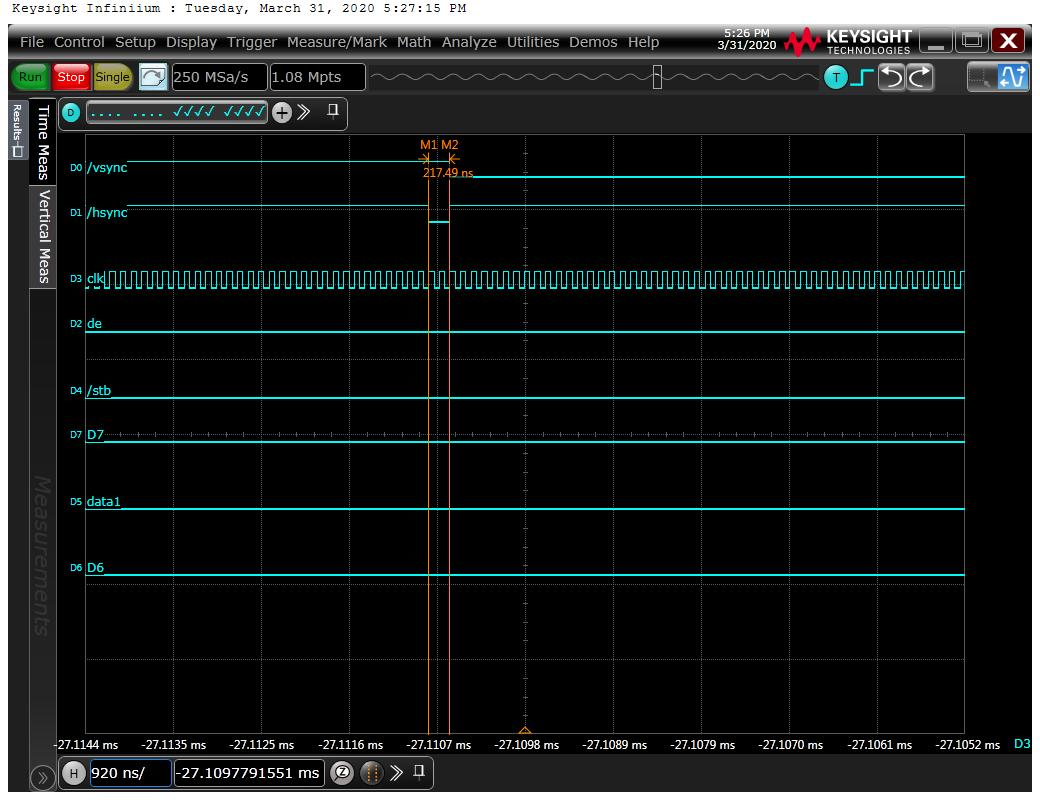
\includegraphics[width=14cm]{pictures/lcd_timings/hsync_length.jpg}
\end{center}
\caption{Length time of one low active H-Sync phase}
\label{fig:hsync_active_time}
\end{figure}

\newpage

\begin{figure}[ht]
\begin{center}
    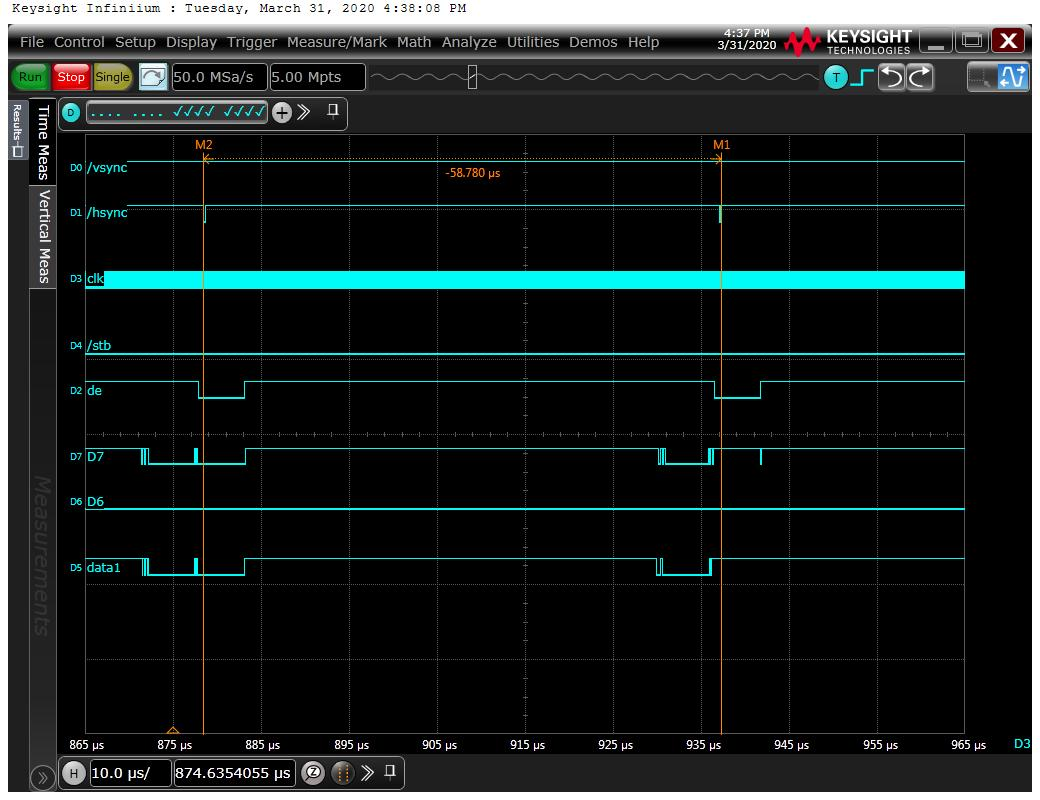
\includegraphics[width=14cm]{pictures/lcd_timings/hsync_periode.jpg}
\end{center}
\caption{Time length of one howl ht-Sync period}
\label{fig:hsync_period}
\end{figure}

\newpage
\section{V-Sync timings}%
The following graphics show the timings by an logic analyzer on the horizontal
signal dataline (V-Sync) after the LCD gets running. V-Sync is an \textit{active
low} dataline.
\label{sub:vsync_timings}
\begin{figure}[!h]
\begin{center}
    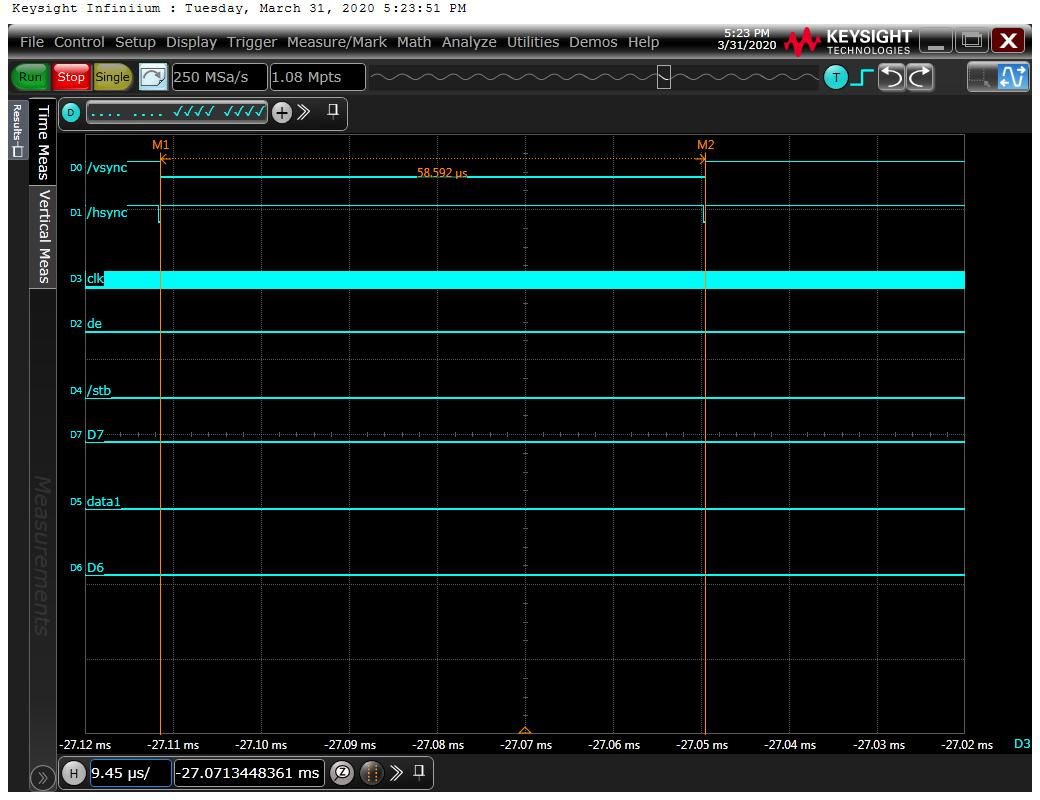
\includegraphics[width=14cm]{pictures/lcd_timings/vsync_length.jpg}
\end{center}
\caption{Length time of one low active V-Sync phase}
\label{fig:vsync_active_time}
\end{figure}
\newpage
\begin{figure}[ht]
\begin{center}
    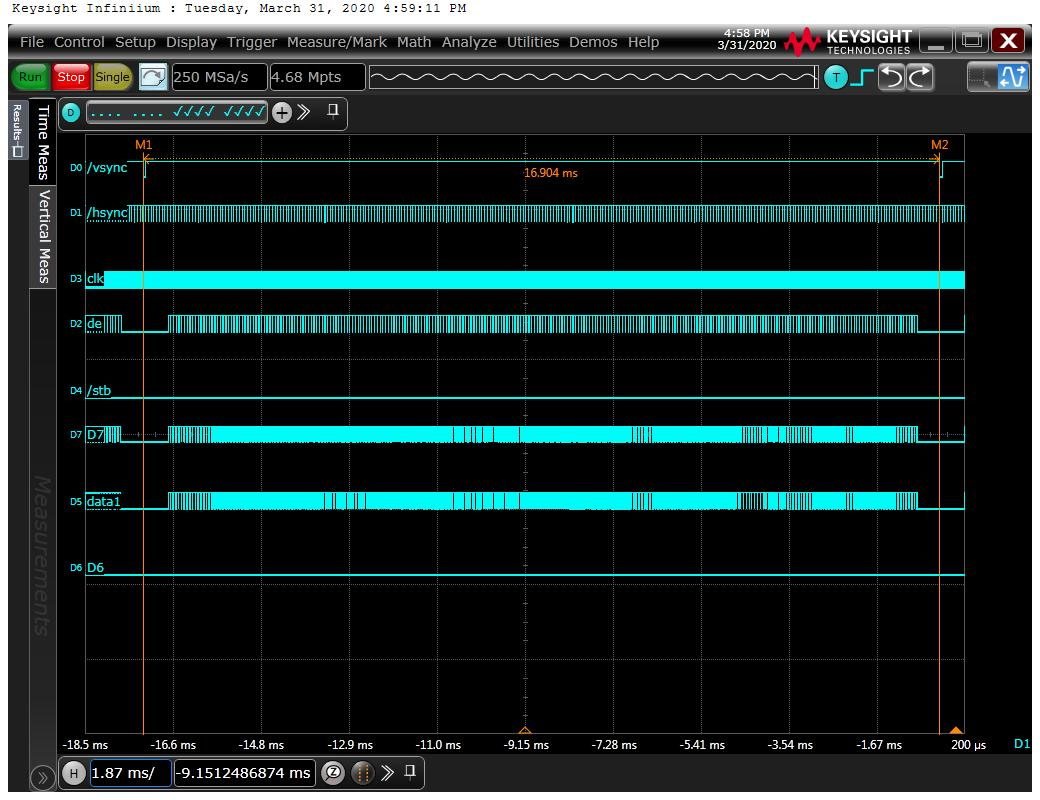
\includegraphics[width=14cm]{pictures/lcd_timings/vsync_periode.jpg}
\end{center}
\caption{Time length of one howl V-Sync period}
\label{fig:one_vsync_period}
\end{figure}

\pagebreak
\section{One Clock time length}%
The following graphics show the timings by an logic analyzer on the clock
after the LCD gets running. Because of falling and rising edge triggering,
timing of clock signal is important.
\label{sub:clock_time_length}
\begin{figure}[h!]
\begin{center}
    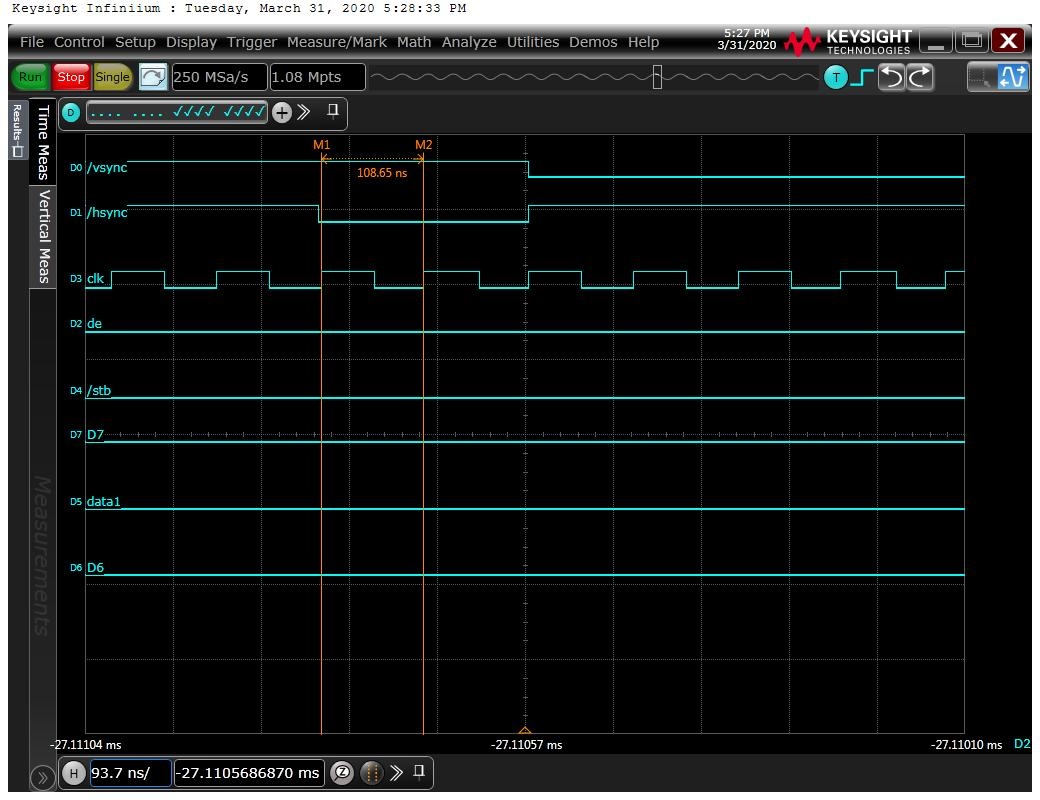
\includegraphics[width=14cm]{pictures/lcd_timings/periode_time_1clk.jpg}
\end{center}
\caption{Time length of one clock period}
\label{fig:one_clock_time}
\end{figure}


\pagebreak
\section{H-Sync vs. DE signal}%
\label{sub:other_measured_lcd_timings}
The following graphics show the timings by an logic analyzer on the H-Sync
signal data line and the data Enable Data line (DE) to get the system
running. Note: The H-Sync is active low and the DE active high both according to
the datasheet and needs to be in time.

\begin{figure}[h!]
\begin{center}
    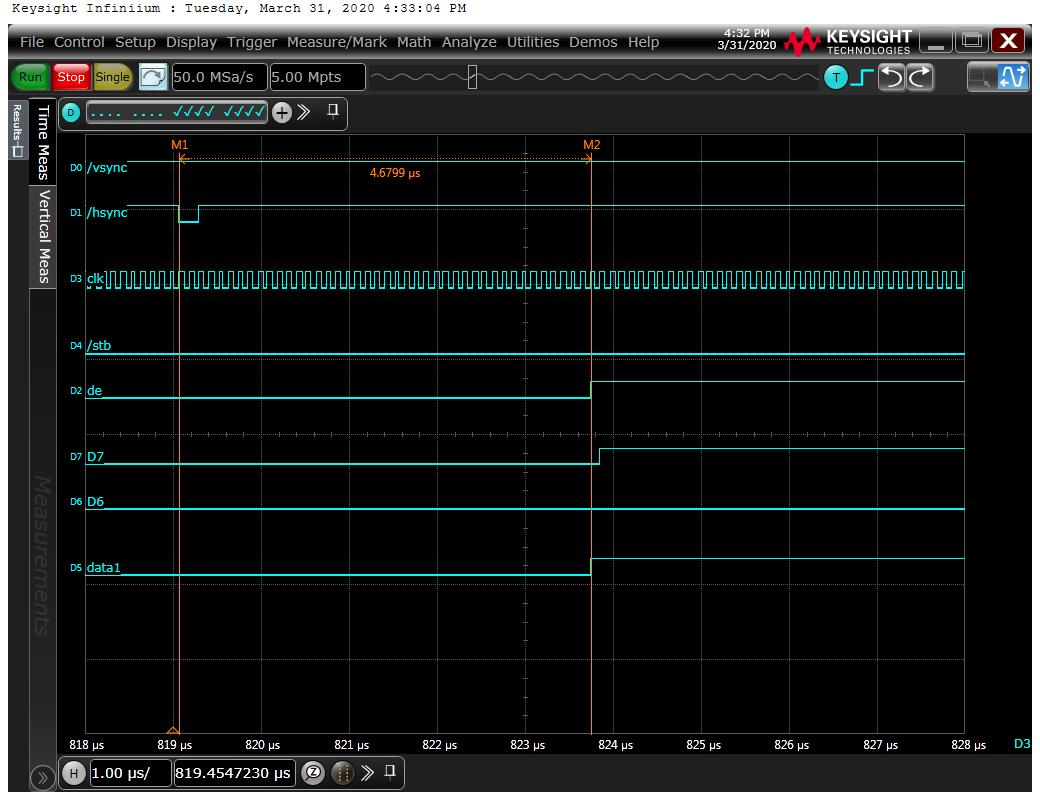
\includegraphics[width=14cm]{pictures/lcd_timings/hsync_falling_de_rising.jpg}
\end{center}
\caption{Time between ht-Sync falling edge and DE rising edge}
\label{fig:hsync_de}
\end{figure}




\chapter{Outlook into the feature}%
\label{cha:ausblick}


\section{U-Boot working with NFS and TFTP}%
\label{sec:uboot_nfstftp}

For further development it would be useful to get an TFTP and NFS server
running. Therefor an Ethernet interface is needed on an development board but
would decrease the development time significantly.

In this case, the bootloader environment needs to be modified to work with your
\gls{TFTP} server and your \gls{NFS} server. Here are some steps needs to be
preformed to get it running

\newpage

\begin{lstlisting}[gobble=4, language=bash,numbers=left,caption=Configure
bootboloader (Barebox or U-Boot) to use NTFS and TFTP.]
         #The bootloader should try to load any image using TFTP
    setenv autoload no

        #The IP of the TFT-Server host. Like 192.168.100.1
    setenv serverip <serverip>

        #Own machine IP address. Like 192.168.100.10
    setenv ipaddr <ipaddr>

        #Networmask bothe machines are in. Like 255.255.255.0
    setenv netmask <netmask>

        #Path to root folder which should be shared
        #ATTATION   NFS share has to set in /etc/exports
        #ATTATION   NFS-Server has to run on the host
    setenv rootpath <rootpath>

        #name of devicetree file to be downloaded
    setenv dtb <dtb>

        #name of the Linux kernel image to be downloaded
    setenv kernel <kernel>

        #Direct start load and start the kernel
        #NOTE   Setting is not needed and not depended to TFTP/NFS
    setenc autostart on

\end{lstlisting}

\newpage

\section{QEMU}%
\label{sec:QEMU}
To decrease the development time a split software from hardware bugs, it would
be useful to simulate the hardware by QEMU.\@ This would make the use of an NFS
and TFTP server possible easy by adding an virtual network adapter.


\chapter{The CP790760 Software}%
\label{cha:software}
The QT4 based Software cargo control software by Telair International GmbH was
taken from the original previous project. Beside some
changes~\ref{sec:software_changes} the software was left untouched.

\section{Software documentation}%
\label{sec:Software_documentation}
This document holds no documentation about the software itself. Documentation
was already preformed by by requirement documentation and is true also for the
software used in this project. No further documentation is needed beside the
software changes in~\ref{sec:software_changes}.


\section{Changes to the Software}%
\label{sec:software_changes}
Mostly the QT4 based Telair Cargo Control Software CP790760 was left untouched.
Nevertheless some changes ware needed to migrate hard coded Linux 3.\@
dependencies to Linux 4.


All changes are preformed by use of C macros inside the original files, whereas
its corespondent values encapsulated into new file inside the software folder
(\fullref{part:location_cp790760_software}).

\begin{alltt}
    \textbf{<cp790760\_softwareroot>/\textbf{linuxversion\_dependencies.h}}
\end{alltt}

\section{Compliance Check and Code Analyze}%
\label{sec:software_anaylse}

The software \textbf{was} tested against functionality. \textbf{Note, no}
other checks were preformed.

\begin{itemize}
    \item The software \textbf{is not} checked by any code analyze tool against
        (possible) bugs or undefined behavior. For example static code analyze.
    \item The software \textbf{is not} checked by any software compliance tool
        against common coding coding rules and guidelines. For example no MISRA
        or CERT.\@
    \item \textbf{No} code reviews were preformed. For example reviews about
        Security or Safety.
\end{itemize}


\section{How to change the Software}%
\label{sec:software_change}
To edit the software sources, change to the software location inside the PTXdist
project. (\fullref{part:location_cp790760_software}). There you can edit the
sources with your favorite editor or \glsshortkey{IDE}. The software can be
compiled by PTXdist.

\subsection{Compile the CP790760 Software}%
\label{sub:compile_CP790760}

PTXDist does not check every single file and folder inside your project against
integrity like manual changes. This would be much to time intensive. That is
why you need to inform PTXDist yourself about your changes.

Therefor first change to you <projectroot> directory and run afterwards:
(See \fullref{part:location_cp790760_software}).


\bigbreak%
\begin{lstlisting}[caption=Mark the CP790760 software as changed]
user@machine:  ptxdist clean telair-cp_790760_1
\end{lstlisting}

Now you can run a software build manual or wait till PTXdist will preformed it
automatically during next generation of howl system images. To build it manual
run from you <projectroot>

\bigbreak%
\begin{lstlisting}[caption=Build the Telair CP790760 software manual]
user@machine:  ptxdist targetinstall telair-cp_790760_1
\end{lstlisting}


Generation of howl images is described in \fullref{sec:final_images_generation}.





% ##################################################
% %Gossary
% ##################################################
%\printglossaries[type=\glsdefaulttype]
\printglossaries{}
\addcontentsline{toc}{chapter}{Glossar}
\addcontentsline{toc}{chapter}{Acronyme}
\cleardoubleemptypage{}

% ##################################################
% Schalgwortverzeichnis (Index)
% ##################################################
\printindex{}



% ##################################################
% Literaturverzeichnis
% ##################################################
\doublespacing{}

\printbibheading{}
%\printbibliography[heading=subbibliography,type=book,title={Books}]
%\printbibliography[heading=subbibliography,type=article,title={Articles}]
\printbibliography[heading=subbibliography,type=online,title={Online resorces}]
%\printbibliography[heading=subbibliography,type=Webpage,title={Online Webpages}]

%\printglossary[type=\acronymtype,title=Abbreviations]
% ##################################################
% Eidesstattliche Erklärung
% ##################################################
% \include{content/affirmation}

%\appendix
% Hier können Anhaenge angefuegt werden

\end{document}
